\documentclass[tikz,border=6pt]{standalone}
\usepackage{amsmath}
\usepackage{newtxtext,newtxmath}
\usetikzlibrary{arrows.meta,calc,decorations.pathreplacing}

\begin{document}
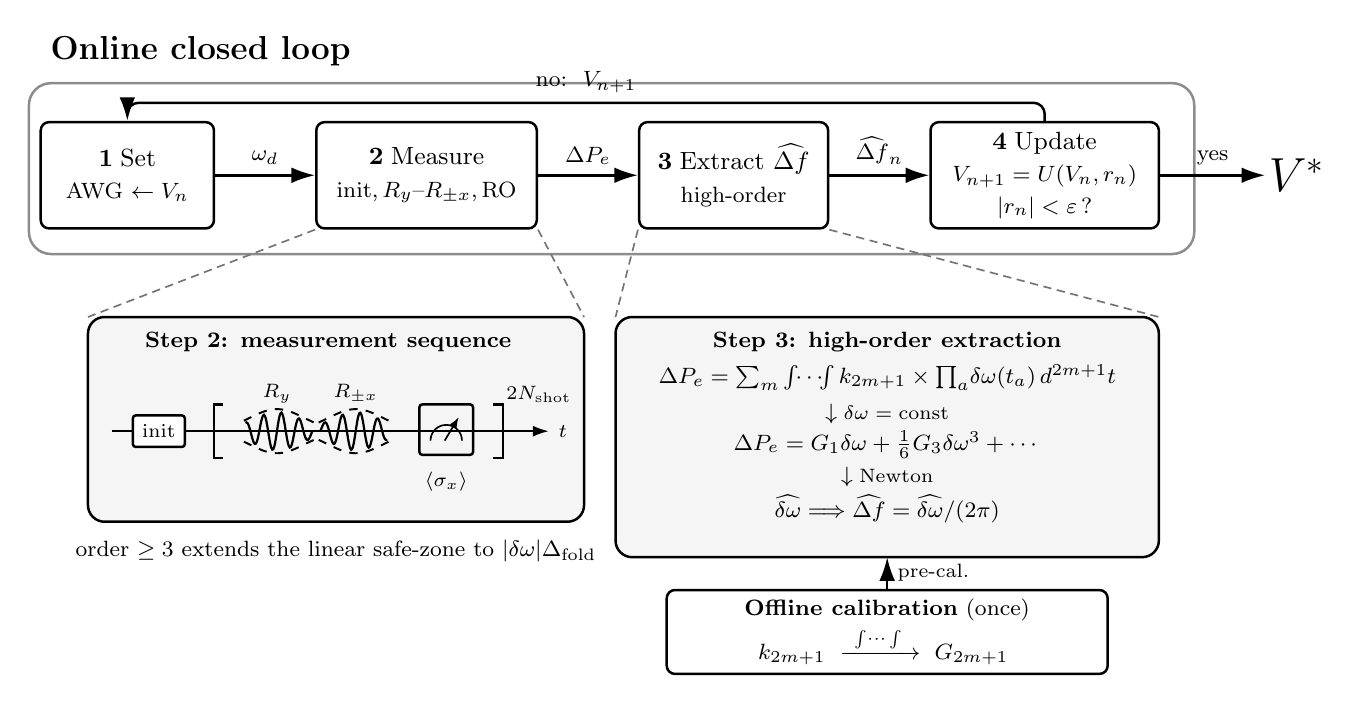
\begin{tikzpicture}[
  x=1cm,
  y=1cm,
  >=Latex,
  font=\large,
  line/.style={draw=black,line width=0.9pt},
  arrow/.style={line,-{Latex[length=3mm,width=2mm]}},
  thinarrow/.style={draw=black,line width=0.55pt,-{Latex[length=2mm,width=1.4mm]}},
  loopbox/.style={line,rounded corners=3pt,align=center,
                  minimum height=1.35cm,font=\small},
  callout/.style={draw=black!55,line width=0.6pt,densely dashed},
  pulse/.style={line,line width=0.8pt},
  envelope/.style={line,dashed,line width=0.7pt}
]

% =====================================================================
% Online closed loop  (host <-> AWG/ADC)   [shifted left to fill corner]
% =====================================================================
\node[font=\bfseries\large,anchor=west] at (2.60,5.62)
  {Online closed loop\quad\mdseries\large};

\draw[line,rounded corners=8pt,draw=black!45] (2.45,3.05) rectangle (17.25,5.22);

\node[loopbox,minimum width=2.2cm] (drive)  at (3.70,4.05)
  {\textbf{1}\;Set\\[0.03cm]{\footnotesize AWG $\leftarrow V_n$}};
\node[loopbox,minimum width=2.8cm] (ramsey) at (7.50,4.05)
  {\textbf{2}\;Measure\\[0.03cm]{\footnotesize init,\,$R_y$--$R_{\pm x}$,\,RO}};
\node[loopbox,minimum width=2.4cm] (extract) at (11.40,4.05)
  {\textbf{3}\;Extract $\widehat{\Delta f}$\\[0.03cm]{\footnotesize high-order }};
\node[loopbox,minimum width=2.9cm] (update) at (15.35,4.05)
  {\textbf{4}\;Update\\[0.03cm]{\footnotesize $V_{n+1}=U(V_n,r_n)$}\\[0.01cm]{\footnotesize $|r_n|<\varepsilon\,?$}};

\draw[arrow] (drive.east)  -- node[above,font=\footnotesize] {$\omega_d$} (ramsey.west);
\draw[arrow] (ramsey.east) -- node[above,font=\footnotesize] {$\Delta P_e $} (extract.west);
\draw[arrow] (extract.east) -- node[above,font=\footnotesize] {$\widehat{\Delta f}_n$} (update.west);

% feedback (no): from update top, over the loop, back into drive
\draw[arrow,rounded corners=4pt]
  (update.north) -- (15.35,4.97) -- (3.70,4.97)
  node[midway,above,font=\footnotesize] {no:\ \ $V_{n+1}$}
  -- (drive.north);

% converged (yes) output -> right, out of the loop band
\draw[arrow] (update.east) -- node[above,font=\footnotesize] {yes} (18.15,4.05);
\node[font=\LARGE] at (18.55,4.05) {$V^\ast$};

% =====================================================================
% Two equal-weight zoom panels, side by side, pulled up close to loop
% =====================================================================
\draw[callout] (ramsey.south west)  -- (3.2,2.25);
\draw[callout] (ramsey.south east)  -- (9.5,2.25);
\draw[callout] (extract.south west) -- (9.9,2.25);
\draw[callout] (extract.south east) -- (16.8,2.25);

% ---------- Panel A : step 2 measurement sequence (hardware init + drive + readout)
\fill[black!4,rounded corners=6pt] (3.2,-0.35) rectangle (9.5,2.25);
\draw[line,rounded corners=6pt]    (3.2,-0.35) rectangle (9.5,2.25);
\node[anchor=north,align=center,font=\footnotesize] at (6.35,2.18)
  {\textbf{Step 2: measurement sequence}\ \ };

% single timeline (doubles as the t axis)
\draw[thinarrow] (3.50,0.80) -- (9.05,0.80) node[right,font=\scriptsize] {$t$};

% global trigger at t0
% \draw[densely dashed,line width=0.6pt] (3.95,0.42) -- (3.95,1.30);
% \fill (3.95,0.80) -- ++(0.16,0.09) -- ++(0,-0.18) -- cycle;
% \node[font=\scriptsize,anchor=south] at (3.95,1.30) {trigger $t_0$};

% repeated single-shot block:  [ |0> . Ry . R+-x . readout ]^{2N_shot}
\draw[line] (4.92,1.14) -- (4.80,1.14) -- (4.80,0.46) -- (4.92,0.46);
\draw[line] (8.35,1.14) -- (8.47,1.14) -- (8.47,0.46) -- (8.35,0.46);
\node[font=\scriptsize,anchor=south west] at (8.39,1.04) {$2N_{\mathrm{shot}}$};

% repetition: loop-back arrow over the bracketed single-shot block
% \draw[-{Latex[length=2mm,width=1.4mm]},line width=0.6pt]
%   (8.57,1.22) .. controls (8.78,1.60) and (4.12,1.60) .. (4.30,1.22);

% init: |0> state preparation / reset
\node[line,fill=white,rounded corners=1pt,minimum width=0.60cm,minimum height=0.40cm,
      font=\scriptsize] at (4.10,0.80) {init};

% two adjacent pi/2 pulses (no free evolution between them)
\node[font=\scriptsize] at (5.60,1.28) {$R_y$};
\begin{scope}[shift={(5.60,0.80)}]
  \draw[pulse,domain=-0.40:0.45,samples=66,smooth]
    plot (\x,{0.24*exp(-5*\x*\x)*sin(deg(28*\x))});
  \draw[envelope,domain=-0.42:0.47,samples=44,smooth] plot (\x,{ 0.28*exp(-4.2*\x*\x)});
  \draw[envelope,domain=-0.42:0.47,samples=44,smooth] plot (\x,{-0.28*exp(-4.2*\x*\x)});
\end{scope}
\node[font=\scriptsize] at (6.60,1.28) {$R_{\pm x}$};
\begin{scope}[shift={(6.60,0.80)}]
  \draw[pulse,domain=-0.45:0.40,samples=66,smooth]
    plot (\x,{0.24*exp(-5*\x*\x)*sin(deg(28*\x))});
  \draw[envelope,domain=-0.47:0.42,samples=44,smooth] plot (\x,{ 0.28*exp(-4.2*\x*\x)});
  \draw[envelope,domain=-0.47:0.42,samples=44,smooth] plot (\x,{-0.28*exp(-4.2*\x*\x)});
\end{scope}

% readout: standard quantum-circuit measurement (meter) symbol
\begin{scope}[shift={(7.75,0.80)}]
  \draw[line,rounded corners=1pt] (-0.34,-0.30) rectangle (0.34,0.34);
  \draw[line,line width=0.6pt] (-0.20,-0.12) arc (180:0:0.20);
  \draw[line,line width=0.6pt,-{Latex[length=1.4mm,width=1.0mm]}]
    (-0.02,-0.12) -- (0.16,0.18);
\end{scope}
\node[font=\scriptsize,anchor=north] at (7.75,0.40) {$\langle\sigma_x\rangle$};

% emphasise: tau = 0, no free evolution between the two pi/2 pulses
% \draw[decorate,decoration={brace,amplitude=3.5pt,mirror},line width=0.5pt]
%   (5.20,0.44) -- (6.76,0.44);
% % \node[font=\scriptsize,anchor=north] at (5.98,0.33) {$\tau{=}0$: no free evolution};

% benefit note (under panel A)
\node[font=\footnotesize,align=center] at (6.35,-0.72)
  {order $\ge 3$ extends the linear safe-zone to $|\delta\omega|\lesssim\Delta_{\mathrm{fold}}$};

% ---------- Panel B : step 3 high-order extraction (host DSP) ----------
\fill[black!4,rounded corners=6pt] (9.9,-0.80) rectangle (16.8,2.25);
\draw[line,rounded corners=6pt]    (9.9,-0.80) rectangle (16.8,2.25);
\node[anchor=north,align=center,font=\footnotesize] at (13.35,2.18)
  {\textbf{Step 3: high-order extraction} \\[0.12cm]
     $\begin{aligned}[t]
       \textstyle\Delta P_e=\textstyle\sum_{m}\int\!\!\cdots\!\!\int k_{2m+1}
                 \times{\textstyle\prod_a}\delta\omega(t_a)\,d^{2m+1}t
      \end{aligned}$\\[0.12cm]
   $\downarrow$\;{\scriptsize $\delta\omega=\mathrm{const}$}\\[0.06cm]
   $\Delta P_e=G_1\delta\omega+\tfrac16 G_3\delta\omega^{3}+\cdots$\\[0.08cm]
   $\downarrow$\;{\scriptsize Newton}\\[0.06cm]
   $\widehat{\delta\omega}\Longrightarrow\widehat{\Delta f}=\widehat{\delta\omega}/(2\pi)$};

% =====================================================================
% Offline calibration: tucked under panel B, fed straight up into step 3
% =====================================================================
\node[line,rounded corners=3pt,align=center,font=\footnotesize,
      minimum width=5.6cm,minimum height=1.0cm] (cal) at (13.35,-1.75)
  {\textbf{Offline calibration} (once)\\[0.04cm]
   $k_{2m+1}\ \xrightarrow{\ \int\cdots\int\ }\ G_{2m+1}$\ \ };
\draw[arrow] (cal.north) -- node[right,font=\scriptsize] {pre-cal.} (13.35,-0.80);

\end{tikzpicture}
\end{document}
